\section{Adapter (Wrapper) Pattern}

We thought to use \textbf{Adapter (Wrapper)} pattern beacuse this allow us to keep the same \textit{client} and make it to comunicate with different types of \textit{services}. The client is the historical database, where we want to write on it, and the services are the external database, from which we want to read on it.

\subsection{Structure}

This implementation uses the object composition principle: the adapter implements the interface of one object and wraps the other one.

\begin{center}
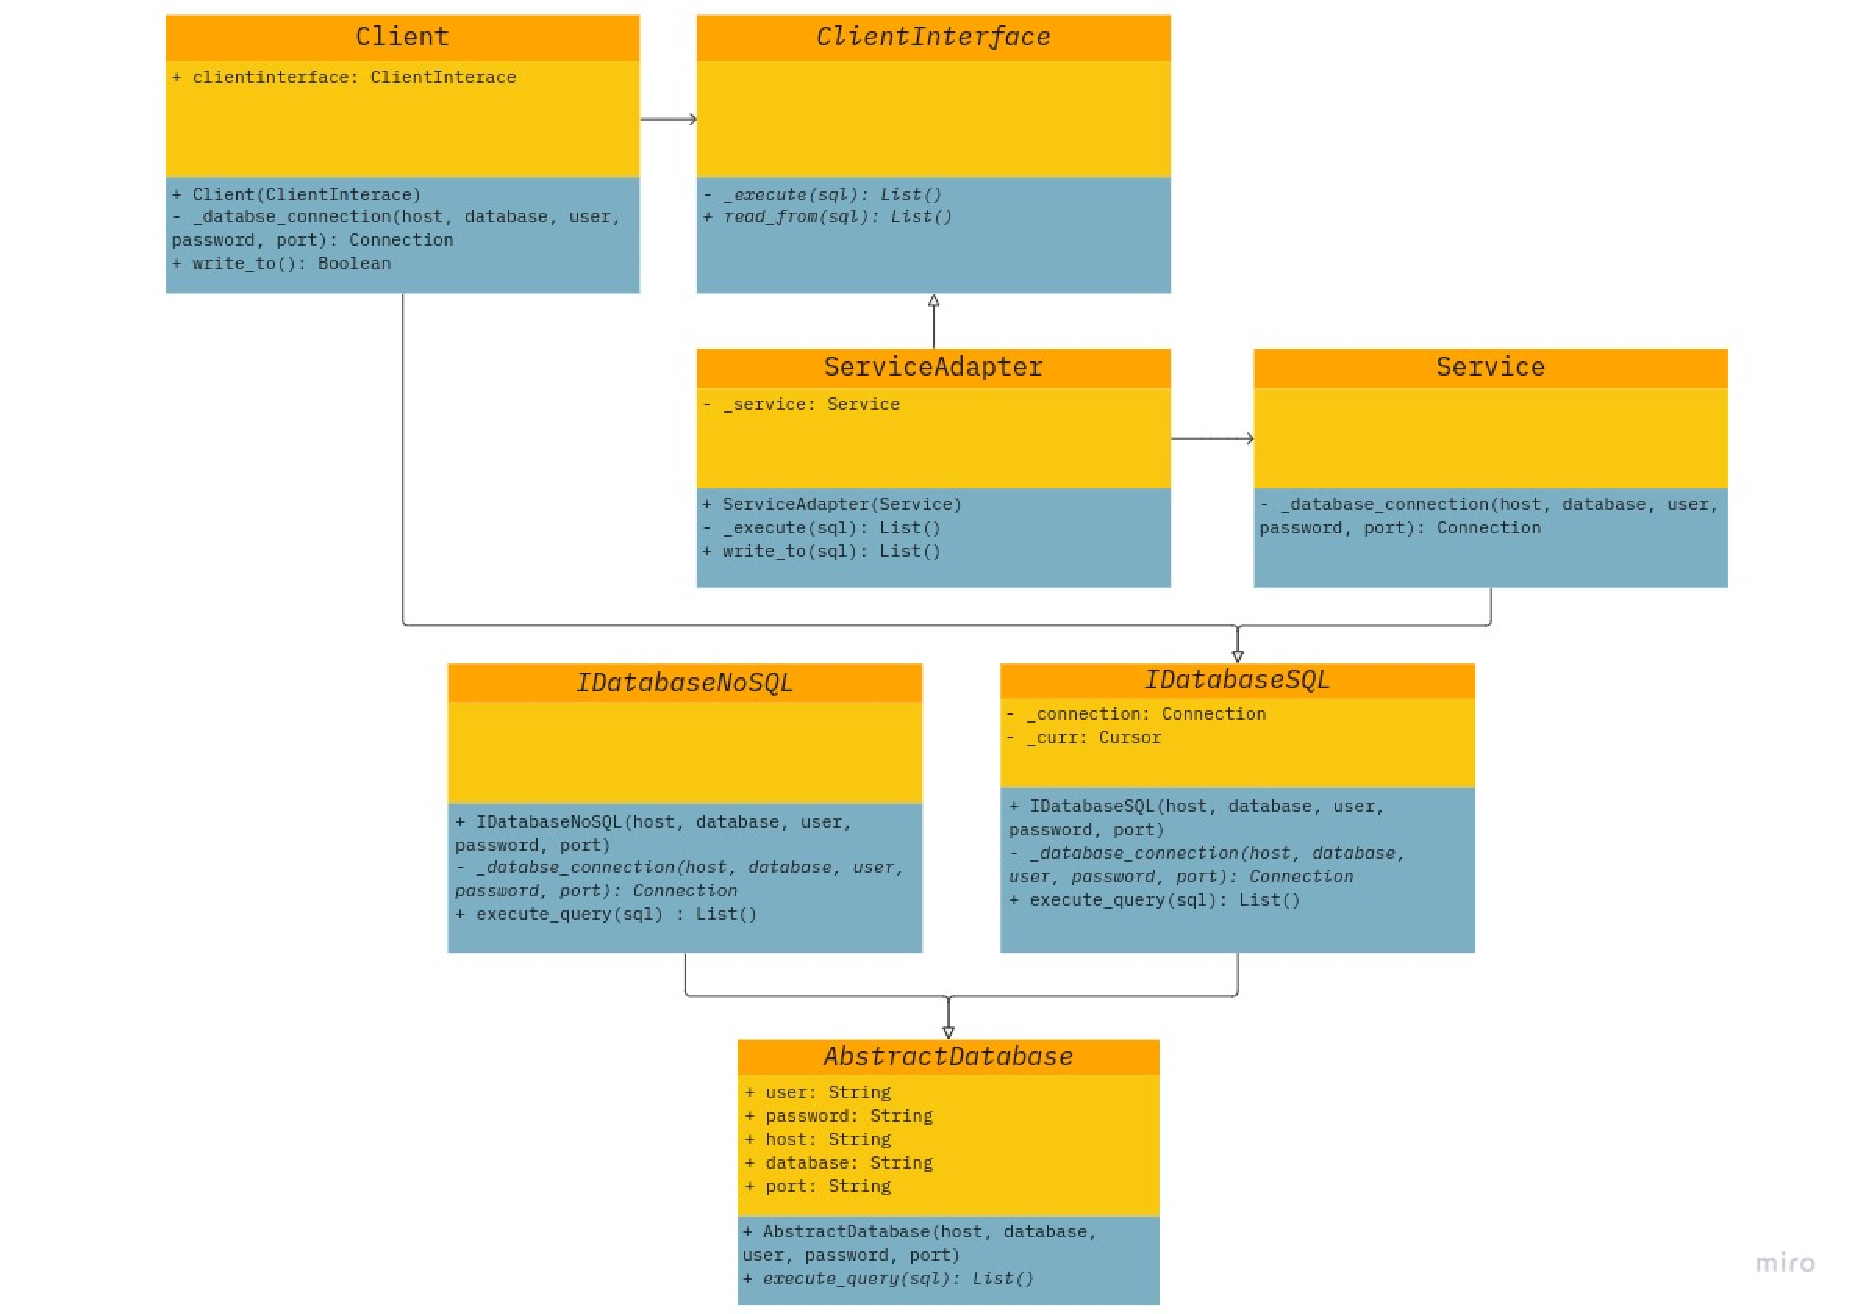
\includegraphics[scale=0.4]{uml-diagram}
\end{center}

\begin{enumerate}
	\item The \textit{AbstractDatabase} is an abstract class that contains data to connect with any database

	\item The \textit{IDatabaseSQL \& IDatabaseNoSQL} are an abstract classes that define behavior of the specified database

	\item The \textit{service} is a concrete class that contains the methods to read from the external database

	\item The \textit{ServiceAdapter} is a concrete class that inherits from \textit{ClientInterface} and contains a \textit{Service} object. Its purpose is to get data from service and make it readable for the client through the implemented \textit{ClientInterface} methods.

	\item The \textit{ClientInterface} is an interface that contains the delcarations of methods defined for each adapters

	\item The \textit{Client} is a concrete class that contains the methods to write in the historical database, to make it, it use the \textit{ClientInterface} methods to read adapted data from the external database.
\end{enumerate}

\section{Software Architecture Pillars}

\subsection{Being the framework for satisfying requirements}

\textbf{Functional}

Our code is able to read from the external database and write to the historical database without any problems.

\textbf{Technical}

We are able to read from any database and any table of them, if the adapters of the databases are setted. And we can write on the historical database if the same table exists and the right fields are setted.

\textbf{Security}

% Our code could be vulnerable by \textbf{sql injection} if the historical and external database
Query precompiled and prepare statement

\subsection{Being the technical basis for design}

% code screenshot

In the our code you can find an interface called \textit{ClientInterface} and its implementation that allows modularization because the \textit{Client} stay unchenged and you could change, add, delete and modify the \textit{Services} as you prefer.

\subsection{Being the managerial basis for cost estimation and process management}
% -------

\subsection{Enabling component reuse}

% code screenshot

Our code is reusable beacuse if you want to change the databse where you read you should only write a new \textit{ServiceAdapter} and \textit{Service} to connect them to the \textit{Client}.

So, if you to use a NoSQL type database, you will implement a new \textit{ServiceAdapter} and \textit{Service} that will inherit from \textit{IDatabaseNoSQL}. Acutally, the most importat thing is that the other part of the code will not change.

\subsection{Allowing a tidy scalability}

Our code allow you to do more INSERT at a time. With an only one Query, thanks to the \textit{ServiceAdapter}, you could read a set of tuples and write them on the historical database with a for loops.

\textbf{TODO:}

In our code is not implemented, but a possibile solution for more scalability is to implement a multi-thread read/write structure.

\subsection{Avoiding handover and people lock-in}

To avoiding handover and people lock-in we could write more comments and documentation about our code.
